
%%%%%%%%%%%%%%%%%%%%%%%%%%%%%%%%%%%%%%%%% 
% Short Sectioned Assignment
% LaTeX Template
% Version 1.0 (5/5/12)
%
% This template has been downloaded from:
% http://www.LaTeXTemplates.com
%
% Original author:
% Frits Wenneker (http://www.howtotex.com)
%
% License:
% CC BY-NC-SA 3.0 (http://creativecommons.org/licenses/by-nc-sa/3.0/)
%
%%%%%%%%%%%%%%%%%%%%%%%%%%%%%%%%%%%%%%%%%

%----------------------------------------------------------------------------------------
%	PACKAGES AND OTHER DOCUMENT CONFIGURATIONS
%----------------------------------------------------------------------------------------

\documentclass[paper=a4, fontsize=11pt]{scrartcl} % A4 paper and 11pt font size

\usepackage[T1]{fontenc} % Use 8-bit encoding that has 256 glyphs
%\usepackage{fourier} % Use the Adobe Utopia font for the document - comment this line to return to the LaTeX default
\usepackage[english]{babel} % English language/hyphenation
\usepackage{amsmath,amsfonts,amsthm} % Math packages
%\usepackage[version=3]{mhchem} % Package for chemical equation typesetting
\usepackage{siunitx} % Provides the \SI{}{} and \si{} command for typesetting SI units
\usepackage{graphicx} % Required for the inclusion of images
%\usepackage{natbib} % Required to change bibliography style to APA
\usepackage{authblk}
\usepackage{indentfirst}
\usepackage{subcaption}
\usepackage{wrapfig}
\usepackage{multirow}
\usepackage{hyperref}
\usepackage{float}
\usepackage{url}
\usepackage{booktabs}
\usepackage{times}

\usepackage{lipsum} % Used for inserting dummy 'Lorem ipsum' text into the template

\usepackage{sectsty} % Allows customizing section commands
\allsectionsfont{\centering \normalfont\scshape} % Make all sections centered, the default font and small caps

\usepackage{geometry}
\geometry{left=2.5cm,right=2.5cm,top=2.5cm,bottom=2.5cm}

\graphicspath{{images/}{figures/}}

\usepackage{fancyhdr} % Custom headers and footers
\pagestyle{fancyplain} % Makes all pages in the document conform to the custom headers and footers
\fancyhead{} % No page header - if you want one, create it in the same way as the footers below
\fancyfoot[L]{} % Empty left footer
\fancyfoot[C]{} % Empty center footer
\fancyfoot[R]{\thepage} % Page numbering for right footer
\renewcommand{\headrulewidth}{0pt} % Remove header underlines
\renewcommand{\footrulewidth}{0pt} % Remove footer underlines
\setlength{\headheight}{13.6pt} % Customize the height of the header

\numberwithin{equation}{section} % Number equations within sections (i.e. 1.1, 1.2, 2.1, 2.2 instead of 1, 2, 3, 4)
\numberwithin{figure}{section} % Number figures within sections (i.e. 1.1, 1.2, 2.1, 2.2 instead of 1, 2, 3, 4)
\numberwithin{table}{section} % Number tables within sections (i.e. 1.1, 1.2, 2.1, 2.2 instead of 1, 2, 3, 4)

\linespread{1.2}

%\setlength\parindent{0pt} % Removes all indentation from paragraphs - comment this line for an assignment with lots of text

%----------------------------------------------------------------------------------------
%	TITLE SECTION
%----------------------------------------------------------------------------------------

\newcommand{\horrule}[1]{\rule{\linewidth}{#1}} % Create horizontal rule command with 1 argument of height

\title{	
	\normalfont \normalsize 
	\textsc{Philipps-Universitaet Marburg, The Department of Physics} \\ [25pt] % Your university, school and/or department name(s)
	\horrule{0.5pt} \\[0.4cm] % Thin top horizontal rule
	\huge XXXXXX XXXXXX: Assignment X \\ % The assignment title
	\horrule{2pt} \\[0.5cm] % Thick bottom horizontal rule
}

\author{Houchen \textsc{Li}} % Your name

\date{\normalsize\today} % Today's date or a custom date

\begin{document}

\maketitle % Print the title

%----------------------------------------------------------------------------------------
%	PROBLEM 1
%----------------------------------------------------------------------------------------

\section{Random Hamiltonians}

As Central Limit Theorem, given a sufficiently large sample size, the samples will follow an approximate normal distribution with the original mean, with all variances being approximately equal to the variance of the population divided by ea wich sample's size.


\vspace{2em}

------ RandomHamiltoniansType1 -------------

What will be happen with vector samples rather than scalar? With random matrix, we will see the eigen value distribution. A matrix $H$ is randomly determined with following consition for elements follow normal distribution.
\begin{equation}
  \mathbb{E}H_{ij} = 0, \quad \mathbb{E}|H_{ij}|^2 = \frac{1}{n} 
\end{equation}

In oder to deal with real eigenvalues, we adopt symmetry condition in the matrix. To generate such a matrix $H$, first we determine a n by n matrix $A$ with random elements from normal distribution.
\begin{equation}
  \label{eq:2}
  A'_{ij} = \frac{A_{ij}}{\sqrt{n}} \times \sqrt{2} \rightarrow H = \frac{A' + A'^{T}}{2}
\end{equation}

Then density of eigenvalue $ \rho(\lambda) = \frac{1}{2\pi}\sqrt{4-\lambda^2} ; \int \rho(\lambda) d \lambda= n$

\vspace{2em}

------ RandomHamiltoniansType2 -------------


From the given question,

\begin{equation}
  \label{eq:2}
  H = \frac{A + A^{T}}{2*\sqrt{2}} \quad \rightarrow  \quad  \mathbb{E}H_{ij} = 0, \quad \mathbb{E}|H_{ij}|^2 = \frac{1}{4}
\end{equation}

\begin{align*}
  &\text{Eigenvalue} \quad h_{i}, \quad \int \rho(h)  dh = n, \quad dh = \sqrt{n/4}d\lambda,  \quad \rho(h) = 1/\sqrt{n}\pi\sqrt{4-(4/n)h^2}\\
&\text{Modified eigenvalue} \quad   x_{i} =  h_{i}/\sqrt{n}, \quad   \rho(h)d h \rightarrow  \rho(x) d x= \frac{2}{\pi}\sqrt{1-x^2} dx\\
\end{align*}

\begin{figure}[ht]
  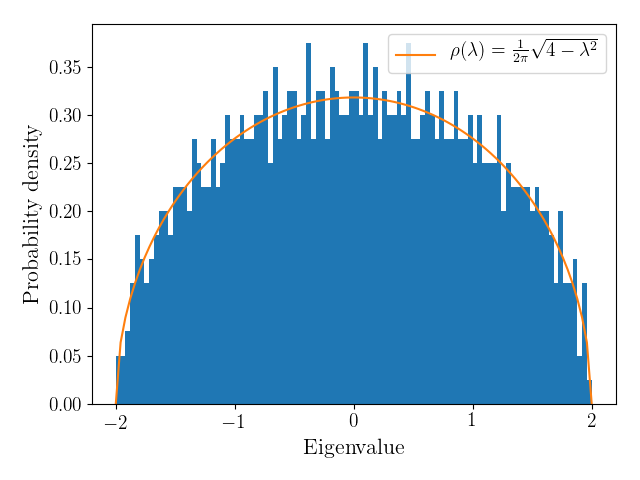
\includegraphics[width = 0.45\textwidth]{figures/figure_7_1_1.png}
  \hfill
  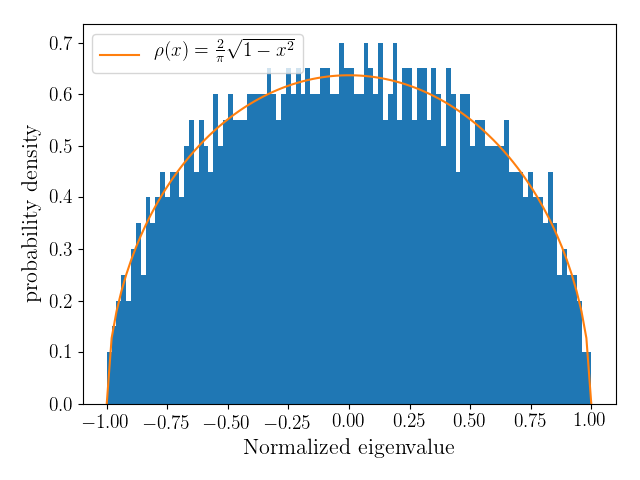
\includegraphics[width = 0.45\textwidth]{figures/figure_7_1_2.png}
  \caption{7.1 eigenvalue density with type1(left) and type2 (right)}
  \label{fig:1}
\end{figure}

Integrated density 

\begin{figure}[ht]
  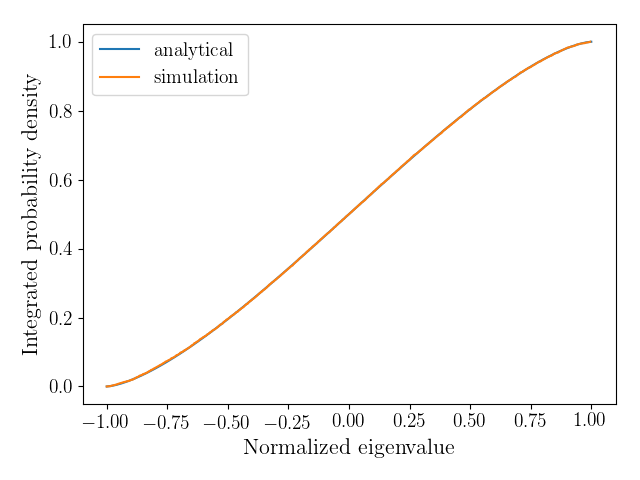
\includegraphics[width = 0.45\textwidth]{figures/figure_7_1_integrated.png}
  \hfill
  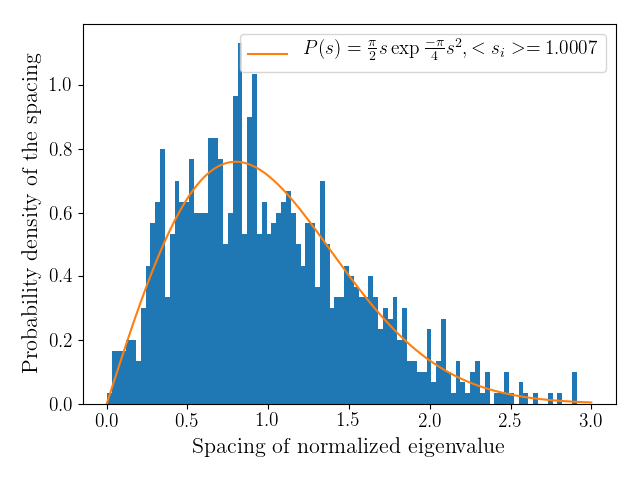
\includegraphics[width = 0.45\textwidth]{figures/figure_7_1_spacing.png}
  \caption{7.1 Integrated density(left) and spacing density(right) of normalized eigenvalues}
  \label{fig:1}
\end{figure}

%----------------------------------------------------------------------------------------
%	PROBLEM 2
%----------------------------------------------------------------------------------------

\section{XXXXXX XXXXXX}

%----------------------------------------------------------------------------------------
%	PROBLEM 2
%----------------------------------------------------------------------------------------

\section{XXXXXX XXXXXX}

%----------------------------------------------------------------------------------------

\end{document}
